\documentclass[12pt]{article}

\usepackage{sbc-template}

\usepackage{graphicx,url}

%\usepackage[brazil]{babel}   
\usepackage[T1]{fontenc}
\usepackage{amsmath,amssymb}
\usepackage{lmodern}
\usepackage[utf8]{inputenc}

     
\sloppy

\title{Utilização da methaeurística GRASP para construção de trilhos de aeronáves}

\author{Alexander A. Pinto\inst{1}, Daniel G. Ramos\inst{1}, Lucídio A. Formiga\inst{1}}


\address{Departamento de Informática -- Universidade Federal da Paraíba (UFPB)\\
  Caixa Postal 5125 -- 58059-900 -- Paraíba -- PB -- Brasil
  \email{\{alex,danielgoncalves\}@lavid.ufpb.br, lucidio@di.ufpb.br}
}

\begin{document} 

\maketitle

\begin{abstract}
  This article discusses the aircraft rotation problem that
concerning the organization of flights planned with the goal of reducing the number
aircraft needed to meet this demand. Obtaining a optimal solution
for this kind of problem ends up being limited because of the nature
combinatorial explosive. We present an algorithm based on metaheuristic
GRASP using the VNS can calculate that in a few
minutes an approximate solution even for large instances. Some
Preliminary results are also presented.
\end{abstract}
     
\begin{resumo} 
Esse artigo descreve o problema de construção de trilhos de aeronaves que se 
refere a organização dos voos planejados com a finalidade de reduzir o número
de aeronaves necessárias para atender essa demanda. A obtenção de uma solução
ótima para esse tipo de problema acaba sendo limitada por causa da natureza 
combinatória explosiva. Apresentamos um algoritmo baseado na metaheurística 
GRASP com a utilização do VNS que consegue calcular em poucos 
minutos uma solução aproximada mesmo para instâncias grandes. Alguns 
resultados preliminares também são apresentados.
\end{resumo}


\section{Descrição do problema}

O problema de construção de trilhos de aeronaves (PCTA) se utiliza da frota atribuída ao conjunto de voos existentes e é caracterizado como sendo um dos principais problemas presentes na industria da aviação. No PCTA o objetivo é a construção, para cada uma das frotas da companhia (e para os voos a elas alocados), de sequências encadeadas de voos que possam ser operados por uma única aeronave\cite{abiliolivro}. Cada uma dessas sequências recebe o nome de trilho.

O sequenciamento dos voos pode ocorrer de 4 formas distintas aqui denominado de arcos. Os arcos do tipo 1 permitem a ligação de voos sem a utilização de atrasos e/ou reposicionamentos. Os arcos do tipo 2 utilizam atrasos mas não o reposicionamento. Os arcos do tipo 3 permitem o sequenciamento com a utilização de um voo de reposicionamento mas sem inserir atraso em nenhum dos voos envolvidos. Os arcos do tipo 4 utilizam-se de atrasos e de um voo de reposicionamento para fazer a ligação entre dois voos.

Para resolver o PCTA, devemos estar cientes de algumas restrições que envolvem tempo e espaço. Por exemplo, um avião não pode partir antes da chegada do vôo que lhe antecede, nem de um local diferente da cidade de destino deste mesmo vôo. Há também a restrição de que um vôo deve permanecer em solo, entre conexões, por um período de tempo que seja suficiente para fazer a troca de passageiros e abastecimento da aeronave e quando for o caso para a troca de tripulação, esse tempo varia de acordo com o aeroporto. O PCTA sofre um grande quantidade de restrições sendo as mais importantes as temporais e geográficas.

Vale ressaltar que na resolução do PCTA deve-se levar em consideração as particularidades especificas de cada companhia aérea como o número de aviões disponíveis na frota, o atraso máximo permitido nos voos, a quantidade máxima de voos que podem sofrer atraso, o número máximo de voos que podem ser cancelados, o número máximo de voos de reposicionamento que podem ser criados entre outros.

Outro aspecto importante diz respeito às restrições de manutenção. Sabe-se que um avião deve ter checagens periódicas. Oportunidades de realizar essas tarefas ocorrem apenas em algumas conexões potencialmente disponíveis. Como consequência, uma sequência de voos deve ser construída de forma que essas restrições não sejam violadas. 

Abaixo na Figura \ref{fig:arpexample} temos dois exemplos de montagem de trilhos feitas a partir de um conjunto fictícios de voos. Cada caixinha representa um voo, onde a parte clara representa o tempo de solo que cada voo deve obedecer e a escura o tempo de voo da cidade de origem para a cidade de destino. As letras A, B, C, D, E representam as cidades e a linha pontilhada indica o tempo de inicio e de termino de cada voo.

\begin{figure}[ht]
\centering
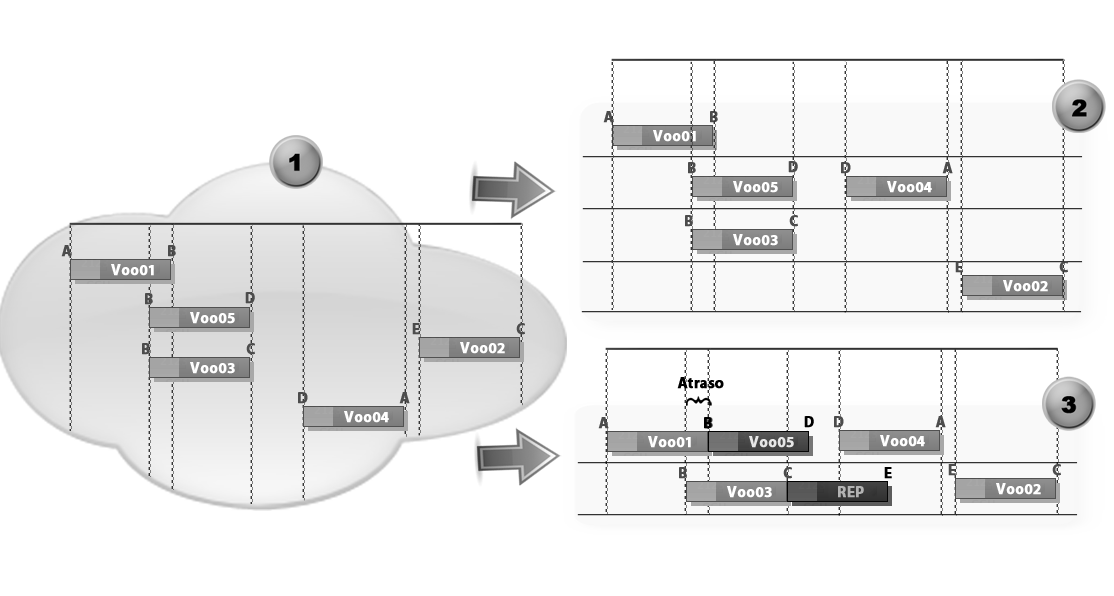
\includegraphics[width=.8\textwidth]{montagemtrilhopeb.png}
\caption{Construção de Trilhos de Aeronaves}
\label{fig:arpexample}
\end{figure}

A parte 1 representa os voos da companhia que ainda não foram cobertos por nenhuma aeronave e nas partes 2 e 3 são demonstrado duas formas de organizar esses voos em trilhos. 

Na parte 2 temos a melhor forma possível de se organizar os voos da parte 1 utilizando apenas os arcos do tipo 1, ou seja sem a utilização de atrasos ou de voos de reposicionamento. Dessa forma se consegue uma formação com 4 trilhos.

Na parte 3 temos a melhor forma de organizar os voos utilizando todos os arcos e um atraso máximo equivalente a um tempo de solo. Dessa forma se consegue uma formação com apenas 2 trilhos.

Pode-se verificar que a utilização de diferentes tipos de arcos pode proporcionar uma melhora significativa  no número de trilhos. Porém essa abordagem faz com que o número de soluções possíveis tenha uma cardinalidade muito superior a utilização de arcos apenas do tipo 1 que por si só já gera uma quantidade de soluções bem elevada, por isso os arcos devem ser utilizados de forma controlada. 


\section{Revisão da Literatura} 


O Trabalho de \cite{arguelo1007} resolve a 
parte de reconstrução de uma solução do PCTA que tenha sido corrompida 
por causa de atrasos e impedimentos de voos que ocorrem durante a 
execução de uma malha. Ele resolve esse problema utilizando a 
metaheurística GRASP, gerando vizinhos da solução atual de forma 
sucessiva até obter uma que seja considerada suficientemente boa.
		
\cite{mercier2007} resolveram o PCTA em 
conjunto com o problema de escala de tripulantes pois 
\cite{cordeau2001}, \cite{klabjan2002} e
\cite{mainville2003} mostraram que a resolução desses problema de 
forma integrada pode gerar soluções que são significantemente melhor 
que as geradas de forma sequencial. 


\section{Proposta do trabalho}

In some conferences, the papers are published on CD-ROM while only the
abstract is published in the printed Proceedings. In this case, authors are
invited to prepare two final versions of the paper. One, complete, to be
published on the CD and the other, containing only the first page, with
abstract and ``resumo'' (for papers in Portuguese).

\section{Resultados preliminares}

Section titles must be in boldface, 13pt, flush left. There should be an extra
12 pt of space before each title. Section numbering is optional. The first
paragraph of each section should not be indented, while the first lines of
subsequent paragraphs should be indented by 1.27 cm.


\bibliographystyle{sbc}
\bibliography{sbc-template}

\end{document}
